%%%%%%%%%%%%%%%%%%%%%%%%%%%%%%%%%%%%%%%%%
% Beamer Presentation
% LaTeX Template
% Version 2.0 (March 8, 2022)
%
% This template originates from:
% https://www.LaTeXTemplates.com
%
% Author:
% Vel (vel@latextemplates.com)
%
% License:
% CC BY-NC-SA 4.0 (https://creativecommons.org/licenses/by-nc-sa/4.0/)
%
%%%%%%%%%%%%%%%%%%%%%%%%%%%%%%%%%%%%%%%%%

%----------------------------------------------------------------------------------------
%	PACKAGES AND OTHER DOCUMENT CONFIGURATIONS
%----------------------------------------------------------------------------------------

\documentclass[
	11pt, % Set the default font size, options include: 8pt, 9pt, 10pt, 11pt, 12pt, 14pt, 17pt, 20pt
	%t, % Uncomment to vertically align all slide content to the top of the slide, rather than the default centered
	%aspectratio=169, % Uncomment to set the aspect ratio to a 16:9 ratio which matches the aspect ratio of 1080p and 4K screens and projectors
]{beamer}

\graphicspath{{Images/}{./}} % Specifies where to look for included images (trailing slash required)

\usepackage{booktabs} % Allows the use of \toprule, \midrule and \bottomrule for better rules in tables
\usepackage{animate}
\usepackage{tikz}
\usepackage{graphicx}
\usepackage{media9}
\usepackage{wrapfig}
\usepackage{multicol}
\usepackage{color}
\setlength{\columnseprule}{1pt}
\def\columnseprulecolor{\color{blue}}
\usepackage{stackengine}
\def\delequal{\mathrel{\ensurestackMath{\stackon[1pt]{=}{\scriptstyle\Delta}}}}


%----------------------------------------------------------------------------------------
%	SELECT LAYOUT THEME
%----------------------------------------------------------------------------------------

% Beamer comes with a number of default layout themes which change the colors and layouts of slides. Below is a list of all themes available, uncomment each in turn to see what they look like.

%\usetheme{default}
%\usetheme{AnnArbor}
%\usetheme{Antibes}
%\usetheme{Bergen}
%\usetheme{Berkeley}
% \usetheme{Berlin}
%\usetheme{Boadilla}
%\usetheme{CambridgeUS}
%\usetheme{Copenhagen}
%\usetheme{Darmstadt}
%\usetheme{Dresden}
% \usetheme{Frankfurt}
%\usetheme{Goettingen}
%\usetheme{Hannover}
%\usetheme{Ilmenau}
%\usetheme{JuanLesPins}
%\usetheme{Luebeck}
\usetheme{Madrid}
% \usetheme{Malmoe}
% \usetheme{Marburg}
% \usetheme{Montpellier}
%\usetheme{PaloAlto}
%\usetheme{Pittsburgh}
%\usetheme{Rochester}
%\usetheme{Singapore}
%\usetheme{Szeged}
%\usetheme{Warsaw}

%----------------------------------------------------------------------------------------
%	SELECT COLOR THEME
%----------------------------------------------------------------------------------------

% Beamer comes with a number of color themes that can be applied to any layout theme to change its colors. Uncomment each of these in turn to see how they change the colors of your selected layout theme.

%\usecolortheme{albatross}
%\usecolortheme{beaver}
%\usecolortheme{beetle}
%\usecolortheme{crane}
%\usecolortheme{dolphin}
%\usecolortheme{dove}
%\usecolortheme{fly}
%\usecolortheme{lily}
%\usecolortheme{monarca}
%\usecolortheme{seagull}
%\usecolortheme{seahorse}
%\usecolortheme{spruce}
%\usecolortheme{whale}
%\usecolortheme{wolverine}

%----------------------------------------------------------------------------------------
%	SELECT FONT THEME & FONTS
%----------------------------------------------------------------------------------------

% Beamer comes with several font themes to easily change the fonts used in various parts of the presentation. Review the comments beside each one to decide if you would like to use it. Note that additional options can be specified for several of these font themes, consult the beamer documentation for more information.

\usefonttheme{default} % Typeset using the default sans serif font
%\usefonttheme{serif} % Typeset using the default serif font (make sure a sans font isn't being set as the default font if you use this option!)
%\usefonttheme{structurebold} % Typeset important structure text (titles, headlines, footlines, sidebar, etc) in bold
%\usefonttheme{structureitalicserif} % Typeset important structure text (titles, headlines, footlines, sidebar, etc) in italic serif
%\usefonttheme{structuresmallcapsserif} % Typeset important structure text (titles, headlines, footlines, sidebar, etc) in small caps serif

%------------------------------------------------

%\usepackage{mathptmx} % Use the Times font for serif text
\usepackage{palatino} % Use the Palatino font for serif text

%\usepackage{helvet} % Use the Helvetica font for sans serif text
\usepackage[default]{opensans} % Use the Open Sans font for sans serif text
% \usepackage[default]{FiraSans} % Use the Fira Sans font for sans serif text
%\usepackage[default]{lato} % Use the Lato font for sans serif text
\usepackage{stmaryrd}
%
%----------------------------------------------------------------------------------------
%	SELECT INNER THEME
%----------------------------------------------------------------------------------------

% Inner themes change the styling of internal slide elements, for example: bullet points, blocks, bibliography entries, title pages, theorems, etc. Uncomment each theme in turn to see what changes it makes to your presentation.

%\useinnertheme{default}
\useinnertheme{circles}
%\useinnertheme{rectangles}
%\useinnertheme{rounded}
%\useinnertheme{inmargin}

%----------------------------------------------------------------------------------------
%	SELECT OUTER THEME
%----------------------------------------------------------------------------------------

% Outer themes change the overall layout of slides, such as: header and footer lines, sidebars and slide titles. Uncomment each theme in turn to see what changes it makes to your presentation.

%\useoutertheme{default}
%\useoutertheme{infolines}
%\useoutertheme{miniframes}
%\useoutertheme{smoothbars}
%\useoutertheme{sidebar}
%\useoutertheme{split}
%\useoutertheme{shadow}
%\useoutertheme{tree}
%\useoutertheme{smoothtree}

%\setbeamertemplate{footline} % Uncomment this line to remove the footer line in all slides
%\setbeamertemplate{footline}[page number] % Uncomment this line to replace the footer line in all slides with a simple slide count

%\setbeamertemplate{navigation symbols}{} % Uncomment this line to remove the navigation symbols from the bottom of all slides

%----------------------------------------------------------------------------------------
%	PRESENTATION INFORMATION
%----------------------------------------------------------------------------------------

\title[Less Regret via Online Conditioning]{Less Regret via Online Conditioning} % The short title in the optional parameter appears at the bottom of every slide, the full title in the main parameter is only on the title page


\author[Sampad Kumar Kar]{Sampad Kumar Kar} % Presenter name(s), the optional parameter can contain a shortened version to appear on the bottom of every slide, while the main parameter will appear on the title slide

\institute[CMI]{\large Chennai Mathematical Institute} 

\date[\today]{\today} % Presentation date or conference/meeting name, the optional parameter can contain a shortened version to appear on the bottom of every slide, while the required parameter value is output to the title slide

%----------------------------------------------------------------------------------------

\begin{document}

%----------------------------------------------------------------------------------------
%	TITLE SLIDE
%----------------------------------------------------------------------------------------

\begin{frame}
	\titlepage % Output the title slide, automatically created using the text entered in the PRESENTATION INFORMATION block above
\end{frame}

%%%%%%%%%%%%%%%%%%%%%%%%%%%%
\logo{
\includegraphics[scale=0.30]{cmi-logo-blue-large.png}~%
}


%%%%%%%%%%%%%%%%%%%%%%%%%%

%----------------------------------------------------------------------------------------
%	TABLE OF CONTENTS SLIDE
%----------------------------------------------------------------------------------------

% The table of contents outputs the sections and subsections that appear in your presentation, specified with the standard \section and \subsection commands. You may either display all sections and subsections on one slide with \tableofcontents or display each section at a time on subsequent slides with \tableofcontents[pausesections]. The latter is useful if you want to step through each section and mention what you will discuss.


%----------------------------------------------------------------------------------------
%	PRESENTATION BODY SLIDES
%----------------------------------------------------------------------------------------

 % Sections are added in order to organize your presentation into discrete blocks, all sections and subsections are automatically output to the table of contents as an overview of the talk but NOT output in the presentation as separate slides

%------------------------------------------------
%---------------------------------------------------------

\section{Introduction}

\begin{frame}{Motivation}
    \begin{itemize}
        \item \emph{Less Regret via Online Conditioning} by Matthew Streeter and H. Brendan McMahan (2010).
        \item We analyze and evaluate an \textbf{Online Gradient Descent} algorithm with adaptive per coordinate adjustment of learning rates.
        \item This leads to regret bounds that are stronger than those of standard online gradient descent for general online convex optimization problems. This is also evident empirically.
    \end{itemize}
\end{frame}

\begin{frame}{Formulation}
    \begin{itemize}
        \item Recall definition of regret in OCO setting:
        $$
        \text{Regret}_T = \sum_{t = 1}^{T} f_{t} (x_t) - \min_{x\in \mathcal{K} } \sum_{t = 1}^{T} f_{t} (x)
        $$
        \item Simplest algorithm that applies to the most general setting of OCO is \textbf{Online Gradient Descent} (OGD) algorithm by Zinkevich (2003). 
    \end{itemize}
\end{frame}

\begin{frame}{Online Gradient Descent}
    \begin{block}{Online Gradient Descent Algorithm}
    \begin{itemize}
        \item Input: Convex Set $\mathcal{K}$, $T$, $x_1 \in \mathcal{K}$, stepsizes $\{\eta_t\}$
        \item for $t = 1$ to $T$ do:
        \begin{itemize}
            \item Play $x_t$ and observe the cost $f_t (x_t)$
            \item Update and Project:
            $$
            \begin{aligned}
                & y_{t+1} = x_t - \eta_t g_t \\
                & x_{t+1} = \Pi_{\mathcal{K}} (y_{t+1})
            \end{aligned}
            $$
            \item Here $g_t$ is a subgradient of $f_t$ at $x_t$.
        \end{itemize}
    \end{itemize}
    \end{block}
\end{frame}

\begin{frame}{OGD Regret Bounds}
    \begin{block}{Theorem 1}
        OGD with stepsize $\{\eta_t = \frac{D}{G\sqrt{t}}, t \in [T]\}$ guarantees the following for all $T \ge 1$:
        $$
        \text{Regret}_T = \sum_{t = 1}^{T} f_{t} (x_t) - \min_{x\in \mathcal{K} } \sum_{t = 1}^{T} f_{t} (x) \le \frac{3}{2} GD\sqrt{T}
        $$
    \end{block}
\end{frame}

\begin{frame}{OGD Regret Bounds}
    \begin{block}{Theorem 1}
        OGD with stepsize $\{\eta_t = \frac{D}{G\sqrt{t}}, t \in [T]\}$ guarantees the following for all $T \ge 1$:
        $$
        \text{Regret}_T = \sum_{t = 1}^{T} f_{t} (x_t) - \min_{x\in \mathcal{K} } \sum_{t = 1}^{T} f_{t} (x) \le \frac{3}{2} GD\sqrt{T}
        $$
    \end{block}
    \textbf{Proof:}
    $$
    \begin{aligned}
        & f_t (x_t) - f_t (x^*) \le \nabla^T f_t (x_t) (x_t - x^*); \text{By Convexity (*)} \\
        & \|x_{t+1} - x^*\|^2 \le \|y_{t+1} - x^*\|^2; \text{By Pythagoras Theorem} \\
        & \nabla^T f(x_t) (x_t - x^*) \le \frac{\|x_t - x^*\|^2 - \|x_{t+1} - x^*\|^2}{2\eta_t} + \frac{\eta_t G^2}{2}; \\
        & \text{By substituting $y_{t+1}$ from OGD (**)}
    \end{aligned}
    $$
\end{frame}

\begin{frame}{Proof}
    $$
    \begin{aligned}
        & f_t(x_t) - f_t (x^*) \le \frac{\|x_t - x^*\|^2 - \|x_{t+1} - x^*\|^2}{2\eta_t} + \frac{\eta_t G^2}{2}; \\
        & \text{using (*) and (**)} \\
        & \text{Regret}_T \le \sum_{t = 1}^{T} \frac{\|x_t - x^*\|^2 - \|x_{t+1} - x^*\|^2}{2\eta_t} + \frac{G^2}{2} \sum_{t = 1}^{T} \eta_t; \\
        & \text{Summing above from $t=1$ to $T$} \\
        & \text{Regret}_T \le \frac{D^2}{2 \eta_T} + \frac{G^2}{2} \sum_{t = 1}^{T} \eta_t; (\dag) \\
        & \text{Regret}_T \le \frac{3}{2} GD\sqrt{T}; \\
        & \text{Assuming $G$- Lipchitz, $D$- Diameter and $\frac{1}{\eta_0} = 0$ and $\eta_t = \frac{D}{G\sqrt{t}}$}
    \end{aligned}
    $$
\end{frame}

\begin{frame}{A Motivating Application}
    \begin{itemize}
        \item \textbf{Problem:} Predicting the probability that a user will click on an ad when it is shown alongside search results for a particular query, using a \textbf{Generalized Linear Model} (GLM):
        \begin{itemize}
            \item On round $t$, Algorithm predicts $p_t(x_t) = l(x_t . \theta_t)$
            \item $x_t, \theta_t \in \mathbb{R}^n$: vector of weights, features, $l$: link function
            \item Ex: $l(\alpha) = \frac{1}{1 + \exp{-\alpha}}$, $l(\alpha) = \alpha$
            \item Algorithm incurs loss, which is some convex function of $p_t$; Ex: cross entropy loss, sum square loss
            \item Played in OGD setting: $x_{t+1} = \Pi_{\mathcal{K}} (x_t - \eta_t g_t)$; $g_t$ being a subgradient of $f_t$ at $x_t$
        \end{itemize}
        \item Single Ad System, we wish to predict it's click-through rate on different queries.
        \item On a large search system, a popular query will occur orders of magnitude more often than a rare query:
        \begin{itemize}
            \item rare queries: need larger learning rates
            \item popular queries: smaller learning rates
        \end{itemize}
    \end{itemize}
\end{frame}

\begin{frame}{Tradeoffs in 1-Dimension: Global Learning Rate}
    \begin{itemize}
        \item Consider $\mathcal{F} = [0,D]$.
        \item When $\eta$ is too \textbf{large}:
            \begin{itemize}
                \item Let $f_t(x) = G |x-\epsilon|$. Then:
                $$
                \nabla f_t(x) = \begin{cases}
                    -G & x \in [0,\epsilon] \\
                    G & x \in (\epsilon, D]
                \end{cases}
                $$
                \item If $x_1 = 0$, then OGD plays\footnote{Assuming $\epsilon < G\eta < D$} $x_t = 0$ on odd rounds and $x_t = G\eta$ on even rounds. Here, $x^* = \epsilon$.
                \item This incurs: $\text{Regret}_T = \frac{T}{2} G \epsilon + \frac{T}{2} G(G\eta - \epsilon) = \frac{T}{2} G^2 \eta$.
                \item Note: The regret is not sublinear.
            \end{itemize}
    \end{itemize}
\end{frame}

\begin{frame}{Tradeoffs in 1-Dimension: Global Learning Rate}
    \begin{itemize}
        \item Consider $\mathcal{F} = [0,D]$.
        \item When $\eta$ is too \textbf{small}:
            \begin{itemize}
                \item Let $f_t(x) = -Gx$. Then $\nabla f_t(x) = -G$
                \item If $x_1 = 0$, then OGD plays $x_t = \min \{D, (t-1)G\eta \}$. Here, $x^* = D$.
                \item Since we are assuming $\eta$ to be small\footnote{For $t < \frac{D}{2 G\eta }$, we have $x_t \le \frac{D}{2}$}:
                \begin{itemize}
                    \item For first $\frac{D}{2G\eta}$ rounds, per round regret is atleast $\frac{GD}{2}$.
                    \item Also\footnote{Assuming $\frac{D}{2G\eta} < T$}, $\text{Regret}_T \ge \frac{GD}{2} \times \frac{D}{2G\eta} = \frac{D^2}{4\eta}$
                \end{itemize}
            \end{itemize}
    \end{itemize}
\end{frame}

\begin{frame}{Tradeoffs in 1-Dimension: Global Learning Rate}
    \begin{itemize}
        \item Consider $\mathcal{F} = [0,D]$.
        \item Based on the above examples, thus for any choice of $\eta$, there exists a problem where ($\ddag$):
        $$
        \max \{\frac{D^2}{4\eta}, \frac{T}{2} G^2 \eta\} \le \text{Regret}_T \le \frac{D^2}{2\eta} + \frac{T}{2} G^2 \eta
        $$
        \begin{itemize}
            \item Upper Bound is adopted from $\textbf{\dag}$\footnote{Substitute a global $\eta_t = \eta$}. By setting $\eta = \frac{D}{G\sqrt{T}}$ (which minimizes the upper bound), we can minimize the worst case regret upto a constant factor\footnote{This leads to a regret bound of $DG\sqrt{T}$}:
            \begin{itemize}
                \item Optimal choice of $\eta$ is proportional to $\frac{D}{G}$
                \item Feasible set is large and gradients are small: large learning rates
                \item Feasible set is small and gradients are large: small learning rates
            \end{itemize}
        \end{itemize}
    \end{itemize}
\end{frame}

\begin{frame}{A Toy Example against Global Learning Rates}
    \begin{block}{Theorem 2}
        There exists a family of online convex optimization problems, parameterized by $T$, where gradient descent with a \textit{non-increasing} \textbf{global learning rate} incurs regret atleast $\Omega(T^{\frac{2}{3}})$, whereas gradient descent with an appropriate \textbf{per-coordinate learning rate} has a regret bound of $\mathcal{O}(\sqrt{T})$
    \end{block}
\end{frame}

\begin{frame}{A Toy Example against Global Learning Rates}
    \begin{block}{Theorem 2}
        There exists a family of online convex optimization problems, parameterized by $T$, where gradient descent with a \textit{non-increasing} \textbf{global learning rate} incurs regret atleast $\Omega(T^{\frac{2}{3}})$, whereas gradient descent with an appropriate \textbf{per-coordinate learning rate} has a regret bound of $\mathcal{O}(\sqrt{T})$. \footnote{This does not contradict the previously stated bound of $\mathcal{O}(GD\sqrt{T})$, as in this family of problems $D = T^{\frac{1}{6}}$ and $G = 1$.}
    \end{block}
    \textbf{Proof:} We interleave the instances of the two classes of $1$-dimensional subproblems discussed previously, by setting $G = 1$ on the feasible set $[0,1]$. Here $\mathcal{F} = [0,1]^{n}$, $n$ is the dimension.
    \begin{itemize}
        \item We have the first subproblem of first type lasting for $T_0$ rounds.
        \item Then we have $C$ subproblems of second type, each lasting for $T_1$ rounds.
    \end{itemize}
\end{frame}

\begin{frame}{Proof (Global Learning Rate)}
    Here is the loss function\footnote{There was a slight typo here in the original paper}:
    $$
    f_t(x_t) = \begin{cases}
        |x_{t,1} - \epsilon| & t \le T_0 \\
        -x_{t,j} & t > T_0 \text{, where } j = 1 + \lceil \frac{t-T_0}{T_1} \rceil
    \end{cases}
    $$
    \begin{itemize}
        \item Each round depends on exactly $1$ coordinate\footnote{So, exactly $1$ component of gradient is non-zero every round}.
        \item As observed from the $1$-dimensional examples, we can easily show that $x^* = (\epsilon, 1, \dots, 1, *, \dots, *)$ \footnote{This is $\epsilon$ followed by $C$ $1$'s, with the remaining elements being irrelevant}. Using this and the bounds obtained from \textbf{$\ddag$} \footnote{For the $1$-D subproblems: $\max \{\frac{D^2}{4\eta}, \frac{T}{2} G^2 \eta\} \le \text{Regret}_T \le \frac{D^2}{2\eta} + \frac{T}{2} G^2 \eta$}:
        \begin{itemize}
            \item $\text{Regret}_T \ge \frac{T_0}{2} \eta + C \min \{\frac{1}{4\eta}, \frac{T_1}{2}\}$
            \item Set $C = T_1 = T_0^{\frac{2}{3}}$ and assume $T_1 \le \frac{1}{2\eta}$
            \item Simple minimization over $\eta$ shows that the sum is $\Omega(T_0^{\frac{2}{3}})$, which is also $\Omega(T^{\frac{2}{3}})$ as $T = T_0 + T_0^{\frac{2}{3}} \le 2T_0$
        \end{itemize}
    \end{itemize}
\end{frame}

\begin{frame}{Proof (Per-Coordinate Learning Rate)}
    So, for gradient descent with \textbf{global learning rate}, we obtain a regret lowerbound of $\Omega(T^{\frac{2}{3}})$.
    \begin{itemize}
        \item We \textit{minimize} the regret upper bounds on a per-coordinate basis. We set the learning rates\footnote{This is what makes this example a per-coordinate learning rate example, because at every iteration exactly one coordinate is meaningfully affected} in the following manner:
        \begin{itemize}
            \item $\eta_t = \sqrt{\frac{1}{T_0}}$ for first $T_0$ rounds and $\eta_t = \sqrt{\frac{1}{T_1}}$ for the remaining $CT_1 + k$ rounds\footnote{This is justified by the fact that we are minimizing the upper bound of $\frac{D^2}{2\eta} + \frac{T}{2} G^2 \eta$ on a per coordinate basis, which gives $\eta^* = \sqrt{\frac{1}{T}}$ for $T$ rounds}.
            \item At this learning rate, we accumulate regret upper bounded by $\sqrt{T}$ for each subproblem of $T$ rounds\footnote{Assuming $D, G = 1$ and $C = T_1 = T_0^{\frac{2}{3}}$}.
            \item Using the  $\text{Regret}_T \le \sqrt{T_0} + C \sqrt{T_1} = 2\sqrt{T_0}$, which means $\text{Regret}_T \in \mathcal{O}(\sqrt{T_0})$ or $\mathcal{O}(\sqrt{T})$.
        \end{itemize}
    \end{itemize}
    So, for gradient descent with \textbf{per-coordinate learning rate}, we obtain a regret upperbound of $\mathcal{O}(\sqrt{T})$.
\end{frame}

\begin{frame}{Improved Global Learning Rate}
    As shown during the proof of \textbf{Theorem 1}, by Zinkevich (2003) showing the regret upper bound of \textit{OGD} at general OCO setting, we have the following:
    $$
    \text{Regret}_T \le \mathcal{B}(\eta_1, \eta_2, \dots, \eta_T) := \frac{D^2}{2 \eta_T} + \frac{1}{2} \sum_{t = 1}^{T} \|g_t\|^2 \eta_t
    $$
    Although the gradients $g_1, g_2 \dots, g_T$ are not known in advance, we can come within a factor of $\sqrt{2}$ on the optimal bound, i.e. $R_{\min}$.\footnote{$R_{\min} := \min_{\eta_1 \le \eta_2 \le \dots \le \eta_T} \mathcal{B}(\eta_1, \eta_2, \dots, \eta_T) = D\sqrt{\sum_{t=1}^{T} \|g_t\|^2}$}

    \begin{block}{Theorem 3}
        Setting $\eta_t = \frac{D}{\sqrt{2 \sum_{i=1}^{t} \|g_i\|^2}}$ yields regret upper bound of $D\sqrt{2 \sum_{t=1}^{T} \|g_t\|^2} = \sqrt{2} R_{\min}$.
    \end{block}
\end{frame}

\begin{frame}{Proof}
    \begin{block}{Theorem 3}
        Setting $\eta_t = \frac{D}{\sqrt{2 \sum_{i=1}^{t} \|g_i\|^2}}$ yields regret upper bound of $D\sqrt{2 \sum_{t=1}^{T} \|g_t\|^2} = \sqrt{2} R_{\min}$.
    \end{block}
    \textbf{Proof:} We first compute the value of $R_{\min}$. As constrained by the proof of \textbf{Theorem 1}, we only consider non-increasing sequences of $\{\eta_t\}$\footnote{If $\eta_t > \eta_{t+1}$ for some $t$, then we can further reduce $\mathcal{B}$ by making $\eta_t$ smaller}.
    \begin{itemize}
        \item This means the bound can be minimized by a constant learning rate $\eta^*$. Simple gradient minimization shows $\eta^* = \frac{D}{\sqrt{2 \sum_{i=1}^{T} \|g_i\|^2}}$, which gives $R_{\min} = D\sqrt{\sum_{t=1}^{T} \|g_t\|^2}$.
    \end{itemize}
    Plugging this choice of $\eta_t$ yields regret upper bound of $\frac{1}{2} D \left( \sqrt{2 \sum_{t=1}^{T} \|g_t\|^2} + \sum_{t=1}^{T} \frac{\|g_t\|^2}{\sqrt{2 \sum_{i=1}^{t} \|g_i\|^2}} \right)$.
\end{frame}

\begin{frame}{Proof}
    We will show that this is upper bounded by $\sqrt{2}R_{\min}$. For this, we use \textbf{Lemma 1}:
    \begin{block}{Lemma 1}
        For $x_1, x_2, \dots x_n \in \mathbb{R}_{\ge 0}$ :
        $$
        \sum_{i = 1}^{n} \frac{x_i}{\sqrt{\sum_{j=1}^{i} x_j}} \le 2 \sqrt{\sum_{i=1}^{n} x_i}
        $$
    \end{block}
    Using \textbf{Lemma 1}, we bound the second term: 
    $$
    \sum_{t=1}^{T} \frac{\|g_t\|^2}{\sqrt{2 \sum_{i=1}^{t} \|g_i\|^2}} \le \sqrt{2 \sum_{t=1}^{T} \|g_t\|^2}
    $$
    This gives an improved regret bound of $\sqrt{2}R_{\min}$.
\end{frame}

% Explain Why this is better than before from (3/2 DGrT) to (rt2 GDrT) here.

%- Per Coordinate Learning Rate Algorithm

\begin{frame}{OGD with per-coordinate learning rate}
    \begin{block}{OGD with per-coordinate learning rate Algorithm}
        \begin{itemize}
            \item Input: Feasible Set $\mathcal{F}$, $T$
            \item Initialize: $x_1 = 0$, $D_i = b_i - a_i$
            \item for $t = 1$ to $T$ do:
            \begin{itemize}
                \item Play $x_t$ and observe the cost $f_t(x_t)$
                \item Update and Project:
                $$
                \begin{aligned}
                    & y_{t+1, i} = x_{t,i} - \eta_{t,i} g_{t,i} \\
                    & x_{t+1} = \Pi_{\mathcal{K}} (y_{t+1})
                \end{aligned}
                $$
                \item Here $x_t$ is a vector whose $i^{th}$ component is $x_{t,i}$ and $g_t$ is a subgradient of $f_t$ at $x_t$.
            \end{itemize}
        \end{itemize}
    \end{block}
\end{frame}

\begin{frame}{OGD Regret Bounds with per-coordinate LRs}
    \begin{block}{Theorem 4}
        Let $\mathcal{F} = \times_{i = 1}^{n}$. Then this Algorithm has regret bounded by $\sum_{i=1}^{n} \mathcal{B}_i \left({\{\eta_{t,i}\}}\right)$, where
        $$
        \mathcal{B}_i \left({\{\eta_{t,i}\}}\right) := D_i^2 \frac{1}{2 \eta_{T,i}} + \frac{1}{2} \sum_{t=1}^{T} g_{t,i}^2 \eta_{t,i} = \sqrt{2}R_{\min,i}
        $$
    \end{block}
\end{frame}

\begin{frame}{Proof}
    \begin{block}{Theorem 4}
        Let $\mathcal{F} = \times_{i = 1}^{n}$. Then this Algorithm has regret bounded by $\mathcal{B} \left({\{\eta_{t}\}}\right) := \sum_{i=1}^{n} \mathcal{B}_i \left({\{\eta_{t,i}\}}\right)$, where
        $$
        \mathcal{B}_i \left({\{\eta_{t,i}\}}\right) := D_i^2 \frac{1}{2 \eta_{T,i}} + \frac{1}{2} \sum_{t=1}^{T} g_{t,i}^2 \eta_{t,i} = \sqrt{2}R_{\min,i}
        $$
    \end{block}
    \textbf{Proof:} Since this algorithm only uses subgradient $g_t$ every iteration, we can assume WLOG that $f_t$ is linear and instead use $f_t^L(x) = g_t.x$, to find a regret upper bound\footnote{This is because $\text{Regret}_{T} \le \text{Regret}_{T}^{L}$, by convexity}.
    \begin{itemize}
        \item Since $\mathcal{F}$ is a hypercube, the projector operator independently projects onto $D_i = [a_i, b_i]$.
        \item This special case is same as solving a separate OCO problem per coordinate $i$, where at $t^{th}$ iteration, the loss function is $f_t^L$.
    \end{itemize}
\end{frame}

\begin{frame}{Proof (cont.)}
    This means for each $i$:
    \begin{itemize}
        \item Set $\eta_t$ such that $\eta_{t,i} = \frac{D_i}{\sqrt{2 \sum_{s=1}^{t} g_{s,i}^2}}$ and by using \textbf{Theorem 3}, we have the following bound \footnote{$R_{\min,i} = \min_{{\{\eta_{t,i}\}}} \{ \mathcal{B}_i \left({\{\eta_{t,i}\}}\right) \}$}:
        $$
        \begin{aligned}
            & \text{Regret}_{T,i}^L := \sum_{t=1}^{T} g_{t,i}x_{t,i} - \min_{y \in D_i} \{ \sum_{t=1}^{T} g_{t,i}y_i \} \\
            & \text{Regret}_{T,i}^L \le \mathcal{B}_i \left({\{\eta_{t,i}\}}\right) = D_i^2 \frac{1}{2 \eta_{T,i}} + \frac{1}{2} \sum_{t=1}^{T} g_{t,i}^2 \eta_{t,i} \\
            & \mathcal{B}_i \left({\{\eta_{t,i}\}}\right) \le D_i\sqrt{2 \sum_{t=1}^{T} g_{t,i}^2} = \sqrt{2}R_{\min,i}
        \end{aligned}
        $$
    \end{itemize}
\end{frame}

\begin{frame}{Proof (cont.)}
    \begin{itemize}
        \item Since $\mathcal{F}$ is a hypercube, this means we collect the combined regret as:
        $$
        \begin{aligned}
            & \text{Regret}_T \le \text{Regret}_T^L = \sum_{i=1}^{n} \text{Regret}_{T,i}^L \\
            & \text{Regret}_T \le \sum_{i=1}^{n} \mathcal{B}_i \left({\{\eta_{t,i}\}}\right) = \sqrt{2} \sum_{i=1}^{n} R_{\min,i} \\
        \end{aligned}
        $$
    \end{itemize}
\end{frame}

%- Show Regret Bound here is better than new global learning rate

\begin{frame}{A tighter Regret Bound}
    \begin{block}{Theorem 5}
        The bounds obtained in \textbf{Theorem 4} is a tighter bound than that obtained in \textbf{Theorem 3}, i.e. we show that\footnote{LHS is the bound obtained by using per-coordinate LR} \footnote{RHS is the improved bound obtained using global LR}
        $$
        \sum_{i=1}^{n} D_i\sqrt{2 \sum_{t=1}^{T} g_{t,i}^2} \le D \sqrt{2 \sum_{t=1}^{T} \|g_t\|^2}
        $$
        where $D = \sqrt{\sum_{i=1}^{n} D_i^2}$ is the diameter of $\mathcal{F}$.
    \end{block}
\end{frame}

\begin{frame}{Proof}
    \begin{block}{Theorem 5}
        $$
        \sum_{i=1}^{n} D_i\sqrt{2 \sum_{t=1}^{T} g_{t,i}^2} \le D \sqrt{2 \sum_{t=1}^{T} \|g_t\|^2}
        $$
    \end{block}
    \textbf{Proof:} Consider vectors $\vec{D} := \{D_i\}_{i=1}^{n}$ and $\vec{G} := \{\sqrt{2 \sum_{t=1}^{T} g_{t,i}^2}\}_{i=1}^{n}$.
    \begin{itemize}
        \item LHS simplifies to $\vec{D}.\vec{G}$
        \item RHS simplifies to $\|\vec{D}\|\|\vec{G}\|$
        \item By \textbf{Cauchy-Schwarz Inequality} $\vec{D}.\vec{G} \le \|\vec{D}\|\|\vec{G}\|$
    \end{itemize}
\end{frame}

\begin{frame}{Experimental Evalutation}
    Online Binary Classification using $2$ recent algorithms for text classification: \textbf{Passive Aggressive} algorithm (PA) and \textbf{Confidence Weighted} algorithm (CW). Here are the results:
    
    \begin{figure}
        \begin{center}
            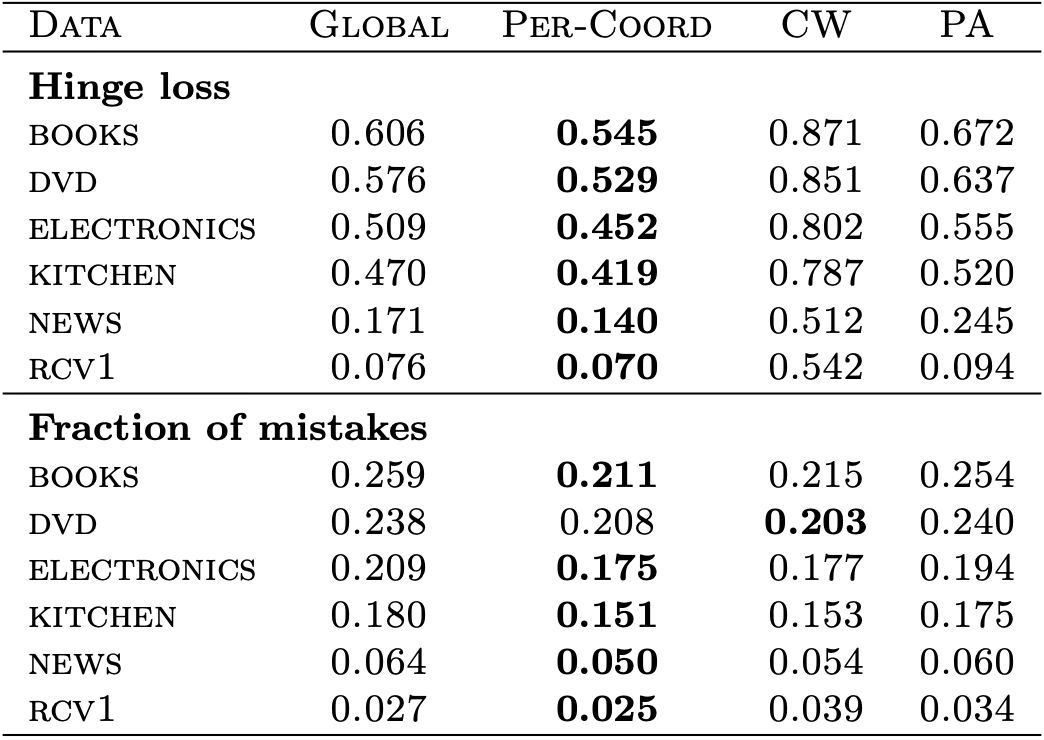
\includegraphics[scale=0.2]{table.jpeg}
        \end{center}
    \end{figure}
\end{frame}

\begin{frame}{Further Exploration}
    \begin{itemize}
        \item For $\alpha$-strongly convex functions we have a regret bound of $\frac{G}{2\alpha}(1 + \log{T})$.
        \item Improved global regret bounds on $\alpha$-strongly convex functions.
        \item Improved per-coordinate regret bounds on $\alpha$-strongly convex functions.
    \end{itemize}
\end{frame}

\begin{frame}{}
    \centering \Large
    \emph{Thank You}
\end{frame}


\end{document}
